\documentclass{tufte-handout}

\title{Session 5}

\author[Pepe García]{Pepe García}

%\date{28 March 2010} % without \date command, current date is supplied

%\geometry{showframe} % display margins for debugging page layout

\usepackage{graphicx} % allow embedded images
  \setkeys{Gin}{width=\linewidth,totalheight=\textheight,keepaspectratio}
  \graphicspath{{../img/}} % set of paths to search for images
\usepackage{listings}  % for code
\usepackage{amsmath}  % extended mathematics
\usepackage{booktabs} % book-quality tables
\usepackage{units}    % non-stacked fractions and better unit spacing
\usepackage{multicol} % multiple column layout facilities
\usepackage{lipsum}   % filler text
\usepackage{fancyvrb} % extended verbatim environments
  \fvset{fontsize=\normalsize}% default font size for fancy-verbatim environments
\usepackage{xcolor}   % for colors

\definecolor{codegreen}{rgb}{0,0.6,0}
\definecolor{codegray}{rgb}{0.5,0.5,0.5}
\definecolor{codepurple}{rgb}{0.58,0,0.82}
\definecolor{backcolour}{rgb}{1,1,1}

\lstdefinestyle{mystyle}{
    backgroundcolor=\color{backcolour},
    commentstyle=\color{codegreen},
    keywordstyle=\color{magenta},
    numberstyle=\tiny\color{codegray},
    stringstyle=\color{codepurple},
    basicstyle=\ttfamily\footnotesize,
    breakatwhitespace=false,
    breaklines=true,
    captionpos=b,
    keepspaces=true,
    numbersep=5pt,
    showspaces=false,
    showstringspaces=false,
    showtabs=false,
    tabsize=4
}

\lstset{style=mystyle}

% Standardize command font styles and environments
\newcommand{\doccmd}[1]{\texttt{\textbackslash#1}}% command name -- adds backslash automatically
\newcommand{\docopt}[1]{\ensuremath{\langle}\textrm{\textit{#1}}\ensuremath{\rangle}}% optional command argument
\newcommand{\docarg}[1]{\textrm{\textit{#1}}}% (required) command argument
\newcommand{\docenv}[1]{\textsf{#1}}% environment name
\newcommand{\docpkg}[1]{\texttt{#1}}% package name
\newcommand{\doccls}[1]{\texttt{#1}}% document class name
\newcommand{\docclsopt}[1]{\texttt{#1}}% document class option name
\newenvironment{docspec}{\begin{quote}\noindent}{\end{quote}}% command specification environment

\begin{document}

\maketitle% this prints the handout title, author, and date

\begin{abstract}
\noindent
In this async session we will learn about functions and then we will
have some exercises to do in order to put in practice all stuff we
have learnt so far.

There is a forum open in Campus, if you feel stuck with anything and
would like to get some help, please post there.  I will check in
several times during the day to answer questions that may pop.
Please, also consider that I will prioritize questions in the forum
before questions you send directly to my email.

If, after reading this handout you feel you want to deepen your
knowledge of Python in general, or functions in particular, you can
try Python for Everybody \cite{py4e}.

Finally, please send over to my email your solutions to the exercises,
they will be considered as homework.  Use a subject line like follows:

\begin{verbatim}
Solutions exercise 5 - <name_and_last_name>
\end{verbatim}

If I had to send it i'd do it with a subject line like this:

\begin{verbatim}
Solutions exercise 5 - Pepe García
\end{verbatim}

\textbf{Do not upload these solutions to Campus} as assignments, just email
them to me.

\end{abstract}

%\printclassoptions

\section{Functions}\label{sec:functions}

Functions are groups of Python statements that have a name and can be
executed on demand.  They will behave as black boxes to which we will
be able to pass data in the form of \textbf{parameters} and that will give
us output in the form of \textbf{return values}.

\begin{marginfigure}%
  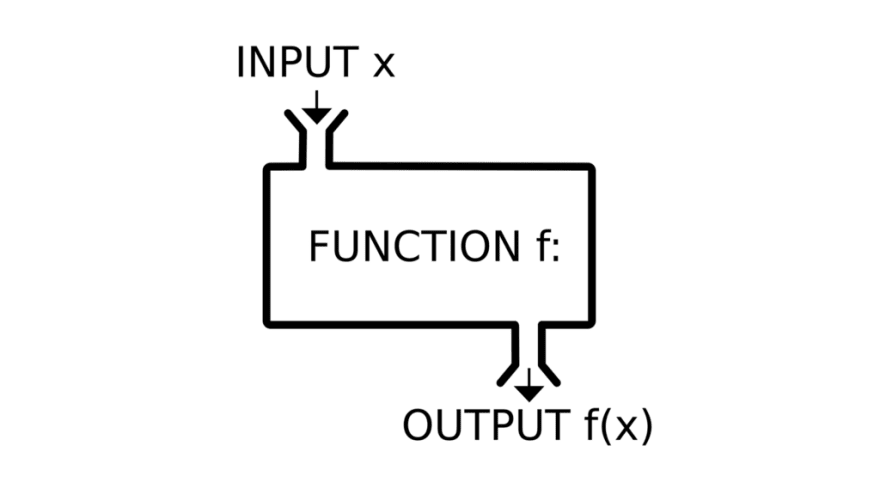
\includegraphics[width=\linewidth]{function.png}
  \caption{Programming functions are similar to mathematical
    functions, they have a domain (\texttt{x} in our example), and a
    codomain (\texttt{f(x)}), and they map values from the domain to
    values in the codomain.}
  \label{fig:marginfig}
\end{marginfigure}

\subsection{Calling functions}\label{sec:callingfunctions}

The syntax for calling functions is the following:

\begin{lstlisting}[language=Python]
function_name(parameter1, parameter2, parameterN)
\end{lstlisting}

When naming functions we will need to apply the same naming rules as
for variables.

We have already seen some functions, such as \textbf{print()},
\textbf{type()}, \textbf{str()}, etc.  We used them as follows:

\begin{lstlisting}[language=Python]
type('hello')
str(3)
int(True)
\end{lstlisting}

Notice that so far, we have used all these functions by passing only
one argument, but there are others that can receive more than one
argument.

\subsection{Declaring functions}\label{sec:declaringfunctions}

We can declare our own functions using the \textbf{def} keyword with the
following syntax:

\begin{lstlisting}[language=Python]
def function_name(parameter1, parameter2):
    #<body>
\end{lstlisting}

When creating a function we need to indent the body to tell Python
what piece of code we want to include inside the function, as we did
with \textbf{if} statements.

\subsection{Returning values from functions}\label{sec:returningvalues}

Functions in Python can return values after doing all the operations
they perform.  In order to return something from a function, we need
to use the \textbf{return} keyword and then pass the value we want to
return.  Here is a simple example of a function that always returns my
name:

\begin{lstlisting}[language=Python]
def return_my_name():
    return 'Pepe'
\end{lstlisting}

\subsection{Function Parameters}\label{sec:functionparameters}

Parameters are values that are injected to the function body when we
call it.  We declare the parameters between the parentheses in the
function definition.

Here's an example of a function used to calculate the area of a
square, that receives a parameter called side, and returns the area.

\begin{lstlisting}[language=Python]
def area_square(side):
    return side * side
\end{lstlisting}

\pagebreak

\section{Exercises}\label{sec:exercises}

\subsection{exercise 1}\label{sec:ex1}

Create a function \Verb|weekly_commute_time| that asks the user their daily
commute time and returns their weekly time spent commuting.

\subsection{exercise 2}\label{sec:ex2}

What do the following expressions return?

\begin{itemize}
\item \Verb|True or 11 > 34|
\item \Verb|False and (1 == 1)|
\item \Verb|(77 // 11) > 6 and False|
\end{itemize}

\subsection{exercise 3}\label{sec:ex3}

Create a function \Verb|area_triangle| that takes the base and height of a
triangle and returns its area

\subsection{exercise 4}\label{sec:ex4}

Create function \Verb|area_triangle_rectangle| that takes the base, height,
and the kind of shape and calculates its area.  It should work for
both triangles and rectangles.

\subsection{exercise 5}\label{sec:ex5}

Create a function \Verb|im_in_love| that takes a weekday number (from
monday to friday), and returns how that weekday is (according to The
Cure!)\footnote{Find some inspiration for this exercise listening to
  them \url{https://www.youtube.com/watch?v=mGgMZpGYiy8}}:

\begin{lstlisting}
I don't care if Monday's blue
Tuesday's grey and Wednesday too
Thursday I don't care about you
It's Friday, I'm in love
\end{lstlisting}

\bibliography{session5}
\bibliographystyle{plainnat}

\end{document}
